\section{Motivation}

% What it is, prevalence
Epilepsy is a neurological condition characterized by abnormal brain activity that gives rise to recurring seizures, affecting about 600 000 people in the UK and 50 million people worldwide \cite{nice_epilepsies_2012,fiest_prevalence_2017}.
This means that around 1\% of the world population live with epilepsy.

% Personal and global burden
Epilepsy is associated with ``stigma, psychiatric comorbidity, and high economic costs'', and it has been ranked by the \ac{WHO} as the second most burdensome neurological disorder in terms of disability-adjusted life years \cite{fiest_prevalence_2017}.
Epileptic seizures, especially repeated, prolonged and uncontrolled tonic-clonic seizures, induce neuronal loss and have long-term behavioral and cognitive consequences \cite{sutula_epileptic_2003}.
The overall risk of dying is 1.6 to 3 times higher in people with epilepsy than in the general population \cite{forsgren_mortality_2005}.
% Deaths in the UK/SUDEP
There are 21 epilepsy-related deaths in the UK every week%
\fnurl{https://sudep.org/epilepsy-deaths},
half of which are \acp{SUDEP}.  % 600/year -> 11.5/week, according to https://epilepsysociety.org.uk/living-epilepsy/sudden-unexpected-death-epilepsy-sudep


\subsection{Video-telemetry and SUDEP}

\ac{SUDEP} is more formally defined as ``the sudden, unexpected, witnessed or unwitnessed, non-traumatic, and non-drowning death in patients with epilepsy with or without evidence for a seizure, and excluding documented status epilepticus, in which postmortem examination does not reveal a structural or toxicological cause for death'' \cite{nashef_sudden_1997}.
It is the most common category of epilepsy-related deaths \cite{devinsky_sudden_2016}.
Although the underlying mechanisms of \ac{SUDEP} are not fully understood, several prognostic risk factors have been identified \cite{so_what_2008, jha_sudden_2021}.
Seizure semiology, the analysis of clinical signs during an epileptic seizure, is an important tool to predict the risk of \ac{SUDEP}.
Some motor semiologies such as decerebration (\cref{fig:decerebration}) have been associated with \ac{PGES}, which has in turn been associated with a higher risk of \ac{SUDEP} \cite{alexandre_risk_2015,vilella_association_2021}.
Therefore, classifying seizures by motor semiologies could be used to assess the risk of \ac{SUDEP} and modify the treatment of epilepsy or give higher priority for surgery to patients with a higher risk.
However, manual assessment of seizure videos by neurophysiologists is time-consuming, as videos can be very long, and presents a high intra- and inter-rater variability, especially between observers from different epilepsy centers \cite{tufenkjian_seizure_2012}.

Our research on automatic classification of seizure videos is presented in \cref{chap:videos}.

\begin{figure}
  \centering

  \begin{subfigure}{0.49\linewidth}
    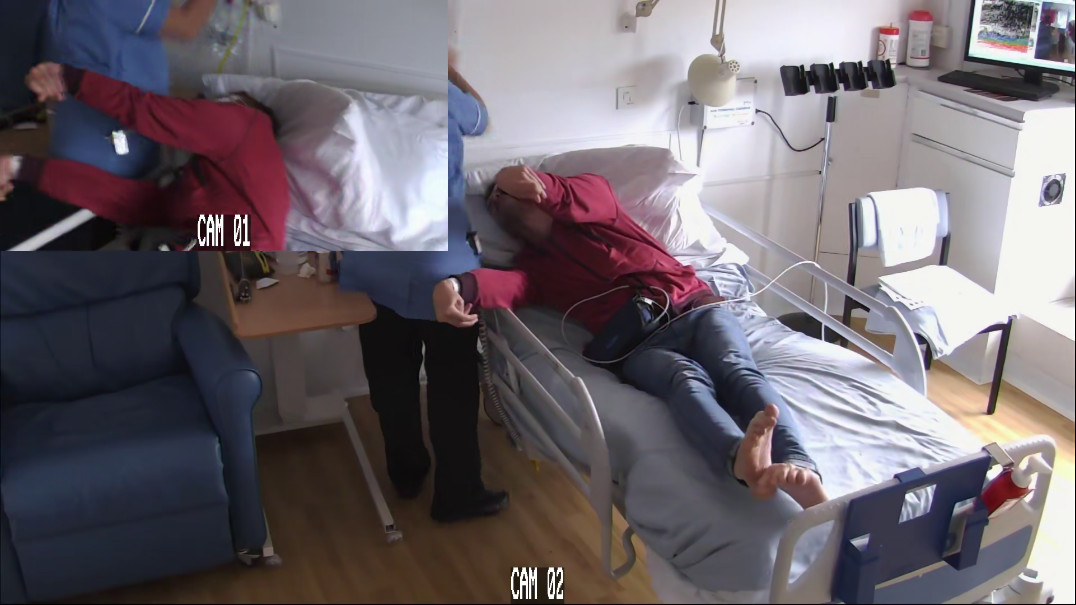
\includegraphics[width=\linewidth]{016_01}
  \end{subfigure}
  \begin{subfigure}{0.49\linewidth}
    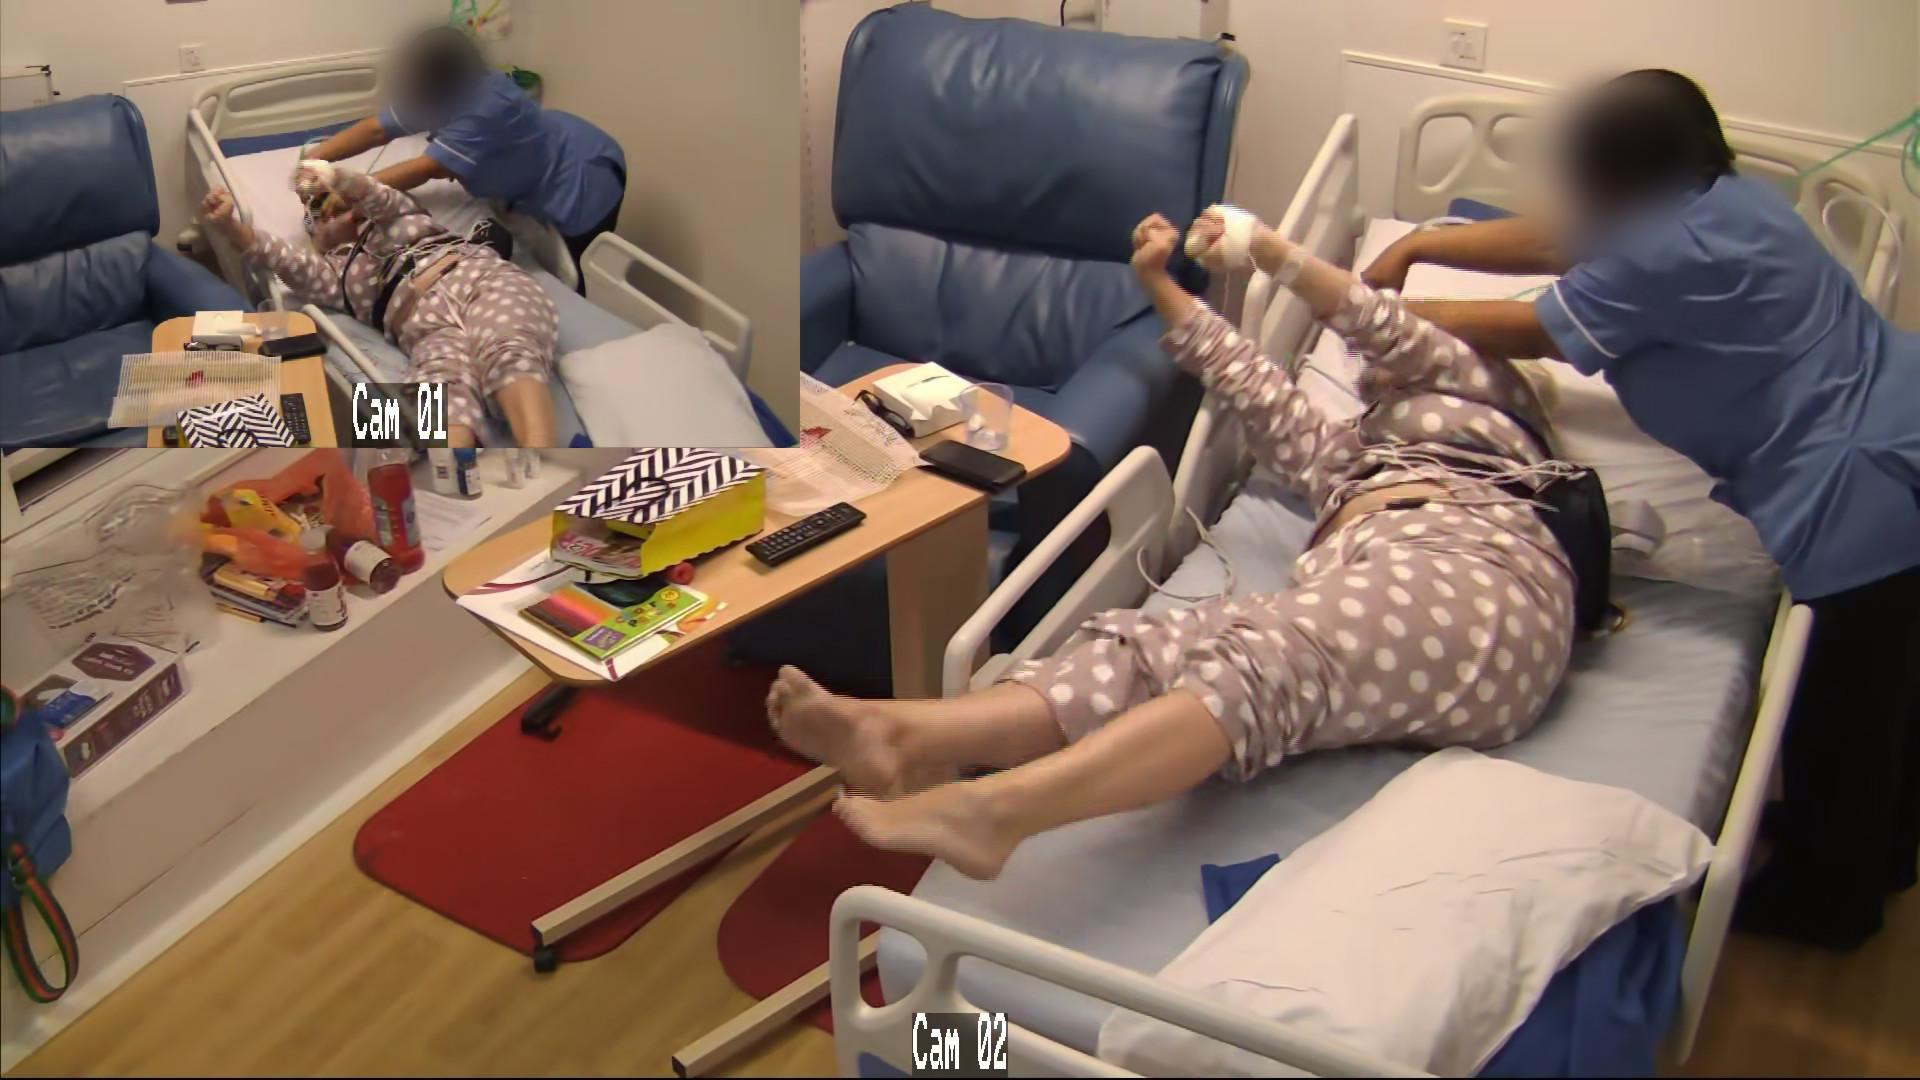
\includegraphics[width=\linewidth]{030_01_blurred}
  \end{subfigure}
  \caption[Examples of decerebrate posturing]{
    Examples of decerebrate posturing during \acp{TCS}.
  }
  \label{fig:decerebration}
\end{figure}


\subsection{Presurgical evaluation}

Antiepileptic drugs are normally used to treat epilepsy.
The aim of these drugs is not to cure the epilepsy, but to decrease the seizure frequency.
In roughly one third of the patients, antiepileptic drugs do not adequately control seizures.
These patients are described as being medically refractory.
Half of the medically refractory epileptic patients have focal epilepsy, which may be treated by curative resective surgery.

The objective of resective epilepsy surgery is the complete resection or complete disconnection of the \ac{EZ}, which is defined as ``the area of cortex indispensable for the generation of clinical seizures'' \cite{rosenow_presurgical_2001}.
The surgery is performed if the \ac{EZ} can be definitely identified and is located in a part of the brain that may be removed without causing neurological, cognitive or neuropsychiatric deficit \cite{jobst_resective_2015}.

To locate the \ac{EZ}, several preoperative imaging scans such as \ac{T1w} \acp{MRI} are acquired in order to identify structural cerebral abnormalities, such as focal cortical dysplasia \cite{kabat_focal_2012}, hippocampal sclerosis \cite{thom_review_2014} or brain tumors.
If a structural lesion is found that is concordant with the results of \ac{EEG} and video-telemetry, the patient can be recommended for surgery after a \ac{fMRI} study to assess language lateralization \cite{duncan_brain_2016}.
However, 15 to 30\% of patients with focal epilepsy are \ac{MRI}-negative, meaning they have no distinct abnormalities visible from imaging or have discordant video \ac{EEG} telemetry \cite{bien_characteristics_2009}.
Results are discordant when they suggest different \ac{EZ} localizations.
For example, an \ac{MRI} can show a lesion near the motor cortex, but \ac{EEG} shows abnormal activity in the occipital lobe.
In such cases, intracranial electrodes may be implanted to acquire \ac{icEEG} signals that for precise localization of the \ac{EZ} (\cref{fig:electrodes}).

\begin{figure}
  \centering
  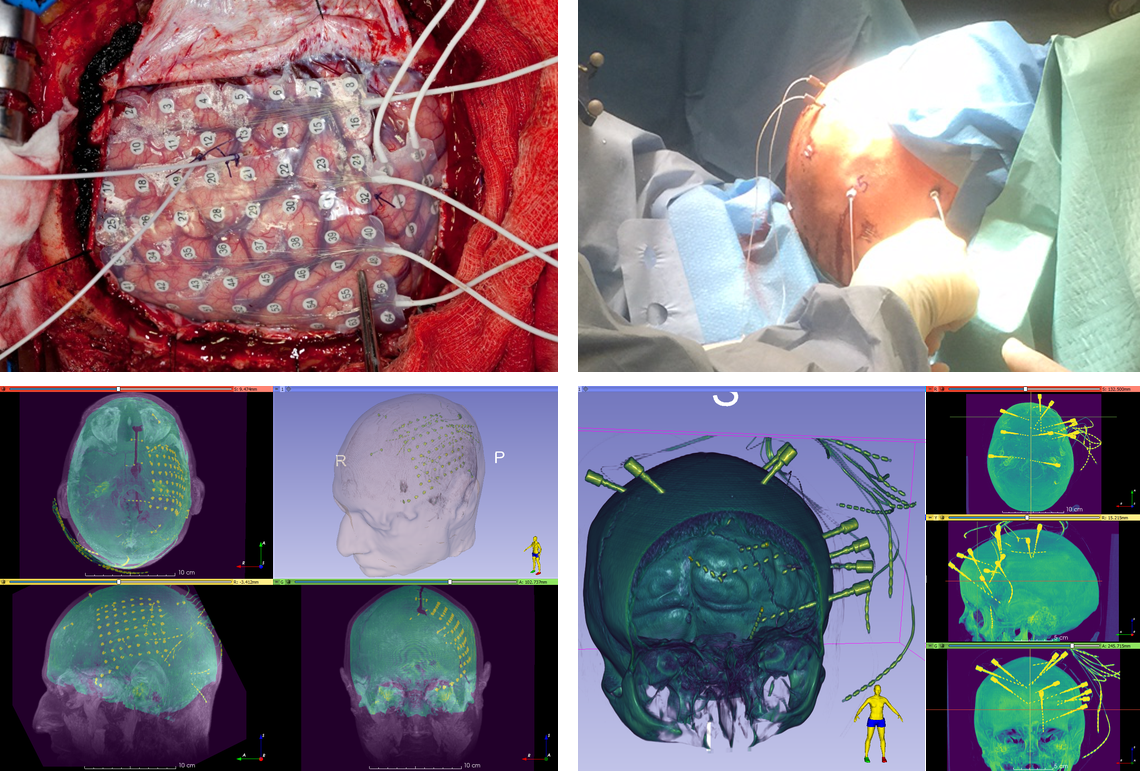
\includegraphics[width=\linewidth]{electrodes}
  \caption[Electrodes used for intracranial EEG]{
    Electrodes used for \ac{icEEG}.
    Left: subdural grid electrode;
    right: \ac{SEEG} depth electrodes.
    Top: intraoperative photos after electrode placement for each implantation procedure;
    bottom: volume renderings and \acp{MIP} of post-implantation images.
    The skull is shown in green. The electrodes and cables are shown in yellow.
  }\label{fig:electrodes}
\end{figure}

The brain structures in which the electrodes are implanted are chosen by clinicians after interpretation of the aforementioned non-invasive data acquisition modalities, particularly seizure semiology, \ac{EEG} and \ac{MRI}.
There are variations in implantation strategies between centers, based on views regarding the relationship between semiological features and brain regions involved.

To determine an objective implantation plan for the \ac{icEEG} electrodes, automatic data-driven methods may be used.
Our tool to objectively map seizure semiologies to brain structures based on the literature is presented in \cref{chap:svt}.


\subsection{Resective surgery}

If the \ac{icEEG} findings enable a definitive localization of the \ac{EZ}, surgery to resect the determined \ac{EZ} may be performed.
Currently, 40\% to 70\% of patients with refractory focal epilepsy are seizure-free%
\footnote{In this context, ``seizure freedom'' refers to one year without seizures from the surgery.}
after surgery \cite{jobst_resective_2015}.
This is, in part, due to limitations identifying the \ac{EZ}.
Retrospective studies relating presurgical clinical features and resected brain structures to surgical outcome provide useful insight to guide \ac{EZ} resection \cite{jobst_resective_2015}.
To quantify resected structures, the resection cavity, which is mostly composed of \ac{CSF} (\cref{fig:cavities}), must be segmented on the postoperative \ac{MRI}.
A preoperative image with a corresponding brain parcellation can then be registered to the postoperative \ac{MRI} to identify resected structures.

3D manual segmentation of brain resection cavities is a time-consuming process requiring highly trained individuals, and a high inter-rater variability is usual \cite{havaei_brain_2017}.
A tool for automatic segmentation would facilitate and accelerate the research to better understand the relation between the clinical features and surgical outcomes.
% However, automatic techniques for cavity segmentation are challenging as other structures in the brain may look similar, such as the ventricles, cysts or oedemas (\cref{fig:}).
% Moreover, brain shift can happen during surgery, creating parts of the images that are also filled with \ac{CSF}.
Our work on automatic segmentation of brain resection cavities is presented in \cref{chap:resection}.


\newcommand{\plotcavities}[2]{
  \begin{subfigure}{0.8\linewidth}
    \includegraphics[trim=0 0 0 50, clip, width=\linewidth]{percentiles/#1}
    \caption{#2}
  \end{subfigure}
}

\begin{figure}
  \centering

  \plotcavities{p_050_0185_without}{Resection cavity in the temporal lobe}
  \plotcavities{p_075_1263_without}{Resection cavity in the frontal lobe}
  \plotcavities{p_025_0039_without}{Resection cavity in the parietal lobe}

  \caption[Examples of brain resection cavities after curative epilepsy surgery.]{
    Examples of brain resection cavities (marked with arrows) after curative epilepsy surgery.
    \textcolor{brown}{TODO: add arrow annotations}
  }
  \label{fig:cavities}
\end{figure}
